
\section{Related Work}
\noindent\textbf{Time Series Foundation Models (TSFMs).} Research has moved from task-specific training to pre-training TSFMs on large corpora for broad transferability. Early work~\cite{rasul2023lag,garza2023timegpt} has advanced to elaborate architectures with patch-based modeling~\cite{ekambaram2024tiny,das2024decoder,goswami2024moment,liu2024timer,liu2024timerxl,liu2025sundial,xiao2025timefound,graf2025flowstate}, sparse mixture-of-experts~\cite{shi2024time,liu2024moirai}, and discretization-based probabilistic objectives~\cite{ansari2024chronos,woo2024unified,ansari2025chronos}. Concurrently, adapting general-purpose large models (LLMs/VLMs) to time series via re-programming or prompting remains active~\cite{zhou2023one,jin2023time,niu2025langtime,sun2025adapting,zhongtime,lyu2025occamvts}. While TSFMs exhibit strong generalization, purely parametric variants perform poorly under severe distribution shifts in downstream domains, demanding effective adaptation strategies~\cite{hinder2024one,jin2022domain,he2023domain}.



% Research has moved from task-specific training to pre-training TSFMs on large corpora for broad transferability. Early work~\cite{rasul2023lag,garza2023timegpt} has advanced to elaborate architectures with patch-based modeling~\cite{ekambaram2024tiny,das2024decoder,goswami2024moment,liu2024timer,liu2024timerxl,liu2025sundial,xiao2025timefound,graf2025flowstate}, sparse mixture-of-experts~\cite{shi2024time,liu2024moirai}, discretization-based objectives~\cite{ansari2024chronos,woo2024unified,ansari2025chronos} and unified probabilistic training~\cite{woo2024unified,ansari2025chronos}. Concurrently, adapting general-purpose large models (LLMs/VLMs)  to time series via re-programming or prompting is still an active research direction~\cite{zhou2023one,jin2023time,niu2025langtime,sun2025adapting,zhongtime,lyu2025occamvts}. While TSFMs exhibit strong generalization, purely parametric variants perform poorly under severe distribution shifts in downstream domains, demanding effective adaptation strategies to mitigate domain gaps~\cite{hinder2024one,jin2022domain,he2023domain}.




\begin{figure*}[t]
  \centering
  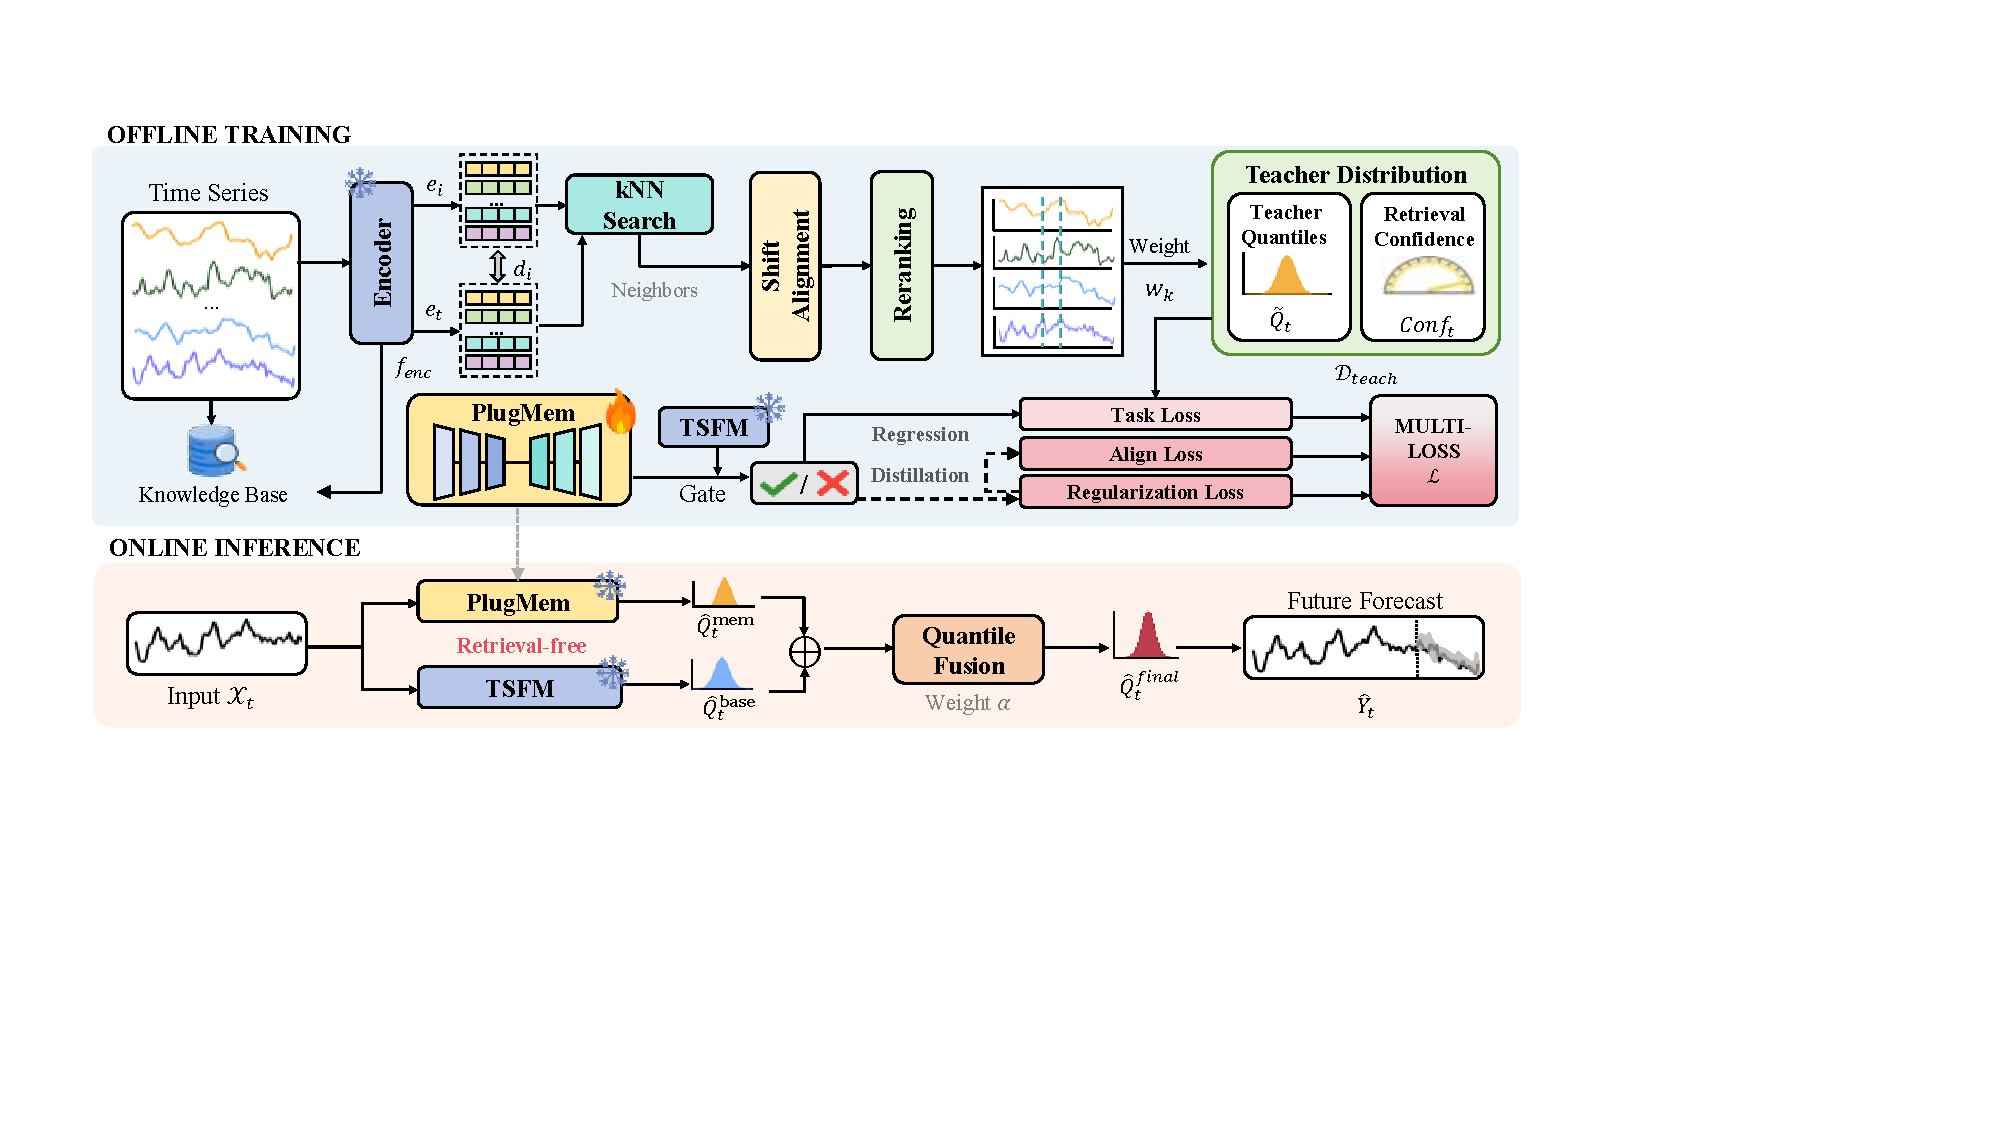
\includegraphics[width=\textwidth]{figures/Overview.pdf}

  \caption{TS-Memory framework. }
  \Description{A two-phase pipeline diagram for TS-PlugMem. }
  \label{fig:ts_plugmem_overview}

\end{figure*}


\noindent\textbf{Adaptation Strategies for TSFMs.} 
To tackle domain shifts, existing work falls into two paradigms: \textit{(1) Parametric adaptation} updates model with target-domain data, ranging from full fine-tuning of all backbone weights, to partial fine-tuning of a small subset of parameters, and parameter-efficient add-ons that keep the backbone frozen while training lightweight modules such as adapters, LoRA-style low-rank updates, or prompt/prefix tuning~\cite{gupta2024low,gupta2024beyond,qiao2025multi,zhao2025less}. While these approaches reduce per-domain training cost, supporting many domains still incurs substantial maintenance overhead~\cite{ning2025mode,lee2025lightweight,sheng2023s}.
% weights (fine-tuning) or input representations (learnable prompts) for target domains~\cite{gupta2024low,gupta2024beyond,qiao2025multi,zhao2025less}, yet suffers from a maintenance trade-off: full fine-tuning leads to high storage costs due to domain-specific model replicas, while continuous shared-backbone updates risk catastrophic forgetting~\cite{ning2025mode,lee2025lightweight,sheng2023s}. 
\textit{(2) Non-parametric retrieval} augments frozen models with external datastore evidence, with lightweight implementations relying on metric-based matching, where query contexts are compared to support embeddings via learned similarity functions for prediction~\cite{koch2015siamese,vinyals2016matching,snell2017prototypical,sung2018learning,oreshkin2018tadam}. For time series, it is commonly realized as subsequence retrieval (via DTW or other distance metrics) followed by aggregation over matched historical windows~\cite{tajmouati2024knn,martinez2019knn,martinez2018dealing,martinez2019tsfknn}. Inspired by NLP's RAG~\cite{lewis2020retrieval}, retrieval augmentation has been adapted to forecasting via relational retrieval, diffusion guidance, LLM-based retrieval and general frameworks~\cite{jing2022retrieval,liu2024retrieval,yang2025timerag,han2025retrieval}, with TSFM systems retrieving context-horizon pairs and fusing retrieved horizons for zero-shot forecasting~\cite{ning2025ts}. Despite their flexibility, these methods introduce heavy search operations into the critical inference path, leading to latency that scales linearly with database size~\cite{fan2024survey}.

We thus propose \textit{(3) Parametric Memory Distillation}. Inspired by memory-augmented networks~\cite{graves2014neural,weston2014memory} and NLP retrieval-free methods~\cite{tay2022transformer,izacard2021distilling}, we distill offline retrieval's distributional knowledge into a lightweight offline module, enabling TS-Memory to achieve retrieval-based adaptability while retaining the constant inference speed and single-model efficiency of frozen TSFMs.

\section{Problem Definition}
\label{sec:setup}

% Let $\mathbf{x}_{1:T} \in \mathbb{R}^{T \times C}$ denote a multi-variate time series with $C$ variables. At time step $t$, we define the \emph{lookback window (context)} as $\mathbf{X}_t = \mathbf{x}_{t-L+1:t} \in \mathbb{R}^{L \times C}$ and the \emph{forecast horizon} as $\mathbf{Y}_t = \mathbf{x}_{t+1:t+H} \in \mathbb{R}^{H \times C}$. We target probabilistic forecasting via \emph{quantiles}. Let $\mathcal{Q}=\{q_k\}_{k=1}^Q$ be the set of target quantile levels, where $q_k\in(0,1)$. 
% % For brevity, we use the multi-index $u=(h,c)$ to represent the $h$-th time step of the $c$-th variable, where $u \in \mathcal{U} = \{1,\dots,H\} \times \{1,\dots,C\}$.
% For brevity, we use the multi-index $u=(h,c)$,where $h \in \{1,...,H\} $ denotes the relative horizon step corresponding to time $t+h$, and $c \in \{1,..,C\}$ denotes the channel.
% Accordingly, $Y_{t,u}$ is the scalar value at time $t+h$ for channel c.

Let $\mathbf{x}_{1:T} \in \mathbb{R}^{T \times C}$ denote a multivariate time series with $C$ channels. At each time step $t$, the \emph{lookback context} $\mathbf{X}_t = \mathbf{x}_{t-L+1:t} \in \mathbb{R}^{L \times C}$ and \emph{forecast horizon} $\mathbf{Y}_t = \mathbf{x}_{t+1:t+H} \in \mathbb{R}^{H \times C}$ are defined accordingly. We target probabilistic forecasting via a set of quantile levels $\mathcal{Q}=\{q_k\}_{k=1}^Q$ with $q_k\in(0,1)$. For brevity, we use the multi-index $u=(h,c)$ where $u \in \mathcal{U} = \{1,\dots,H\} \times \{1,\dots,C\}$, so that $Y_{t,u}$ denotes the scalar value at time $t+h$ for channel $c$.

\noindent\textbf{Frozen Backbone.}
Let $f_{\theta}$ be a pre-trained TSFM with parameters $\theta$.
Given input $\mathbf{X}_t$, it outputs base quantile predictions:
\begin{equation}
    \widehat{\mathbf{Q}}^{\text{base}}_t = f_{\theta}(\mathbf{X}_t) \in \mathbb{R}^{Q \times H \times C}.
    \label{eq:tsm-base-quantile}
\end{equation}
Crucially, to preserve general knowledge and avoid storage overhead, $\theta$ remains frozen throughout the adaptation phase.

\noindent\textbf{Parametric Memory Module.}
We introduce \textbf{PlugMem}, a lightweight, learnable module $g_{\phi}$, parameterized by $\phi$.
It maps the same context $\mathbf{X}_t$ to a complementary set of quantile estimates:
\begin{equation}
    \widehat{\mathbf{Q}}^{\text{mem}}_t = g_{\phi}(\mathbf{X}_t) \in \mathbb{R}^{Q \times H \times C}.
    \label{eq:tsm-mem-quantile}
\end{equation}
Our objective is to optimize $\phi$ to distill retrieval-based distributional knowledge into $\widehat{\mathbf{Q}}^{\text{mem}}_t$, thereby achieving domain adaptation without accessing external databases during inference.
